\begin{frame}
  \frametitle{Mesh adaptation can yield more accurate
  results with less computational resources}
  \begin{columns}
    \begin{column}{0.6\textwidth}
      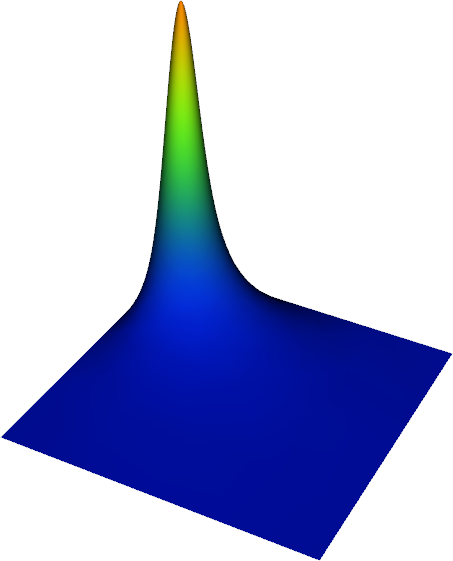
\includegraphics[width=0.9\textwidth]{png/exact-solution-alpha.png}
    \end{column}
    \begin{column}{0.4\textwidth}
    \end{column}
  \end{columns}
\end{frame}
%
\begin{frame}
  \frametitle{Mesh adaptation can yield more accurate
  results with less computational resources}
  \begin{columns}
    \begin{column}{0.6\textwidth}
    \only<1>{
      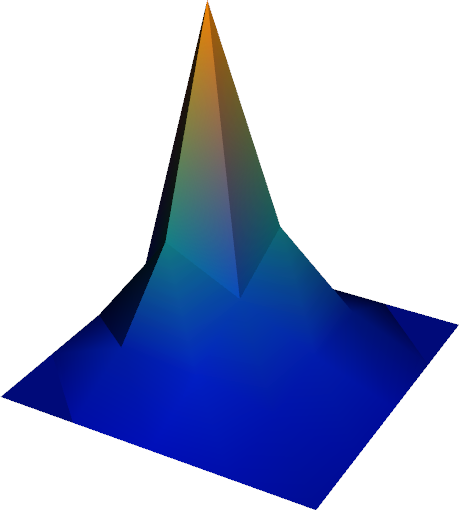
\includegraphics[width=0.9\textwidth]{png/solution-refinement-1.png}
    }
    \only<2>{
      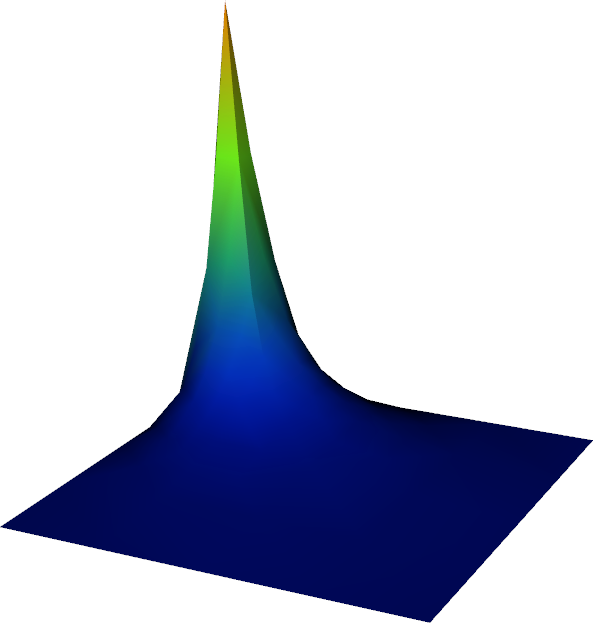
\includegraphics[width=0.9\textwidth]{png/solution-refinement-2.png}
    }
    \only<3>{
      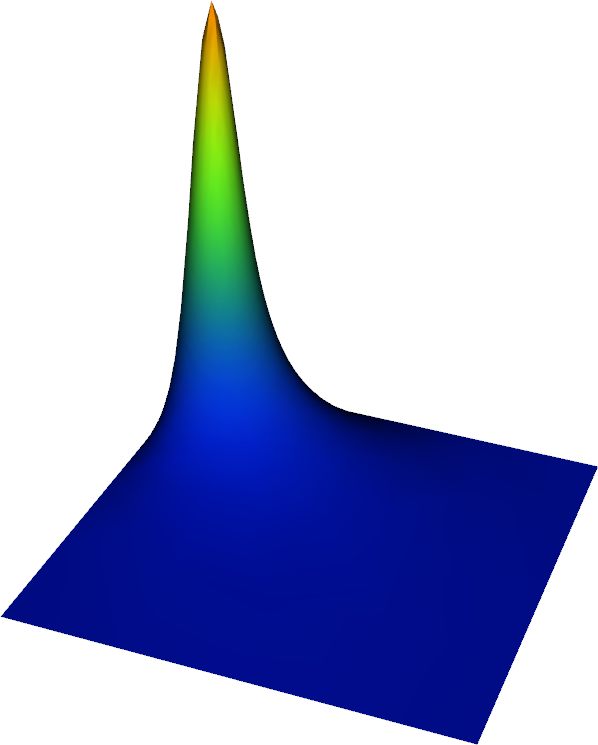
\includegraphics[width=0.9\textwidth]{png/solution-refinement-3.png}
    }
    \end{column}
    \begin{column}{0.4\textwidth}
      \multiinclude[graphics={width=1.0\textwidth,angle=-90},format=pdf,start=1]{pdf/mesh-refinement}
    \end{column}
  \end{columns}
\end{frame}

%  Start with introductory figure again. explain concept
%  of a posteriori estimate for both error assement
%  and driving refinement
%  \\
%  h vs. p refinement (or both)
%  need for error indicators, how do they look like
%  \\
%  they something about the advantage of DF for refinement 
%  and higer order elements
%  \\give versions of error indicators
%  \\mention work from Stamm 1, Houston (2 papers)
%  \\mention efficiency vs reliability
